\section{Da model}
\label{sec:dsmc_model}
DSMC be a model dat make full use of statistical mechanics n' tha kinetic theory of gases. Da physical system consistz of $N$ atomz of tha same type up in a funky-ass box wit volume $V = L_xL_yL_z$ ($L_i$ bein tha length of tha box up in tha $i'$th dimension) n' porositizzle $\phi$ (the porositizzle was tha fraction of tha total volume available fo' fluids). Da atoms all have mass $m$ n' a effectizzle diameter $d$. Instead of trackin tha trajectory every last muthafuckin single atom, we simulate $M$ particles, each representin $N_\text{eff}$ real atoms. We can interpret dis approximation as dat all atoms up in a lil' small-ass region of space round tha coordinatez of a simulated particle move wit approximately tha same velocity. Da system is periodic up in all directions which means dat $(L_x, L_y, L_z) = (0,0,0)$, tha cornerz of tha cube is tha same point. If a particle passes all up in a funky-ass boundary surface (one of tha sidez of tha box), it will just enter all up in tha opposite side, peep figure \ref{fig:dsmc_periodic_boundary_conditions}.
\begin{figure}[ht]
\begin{center}
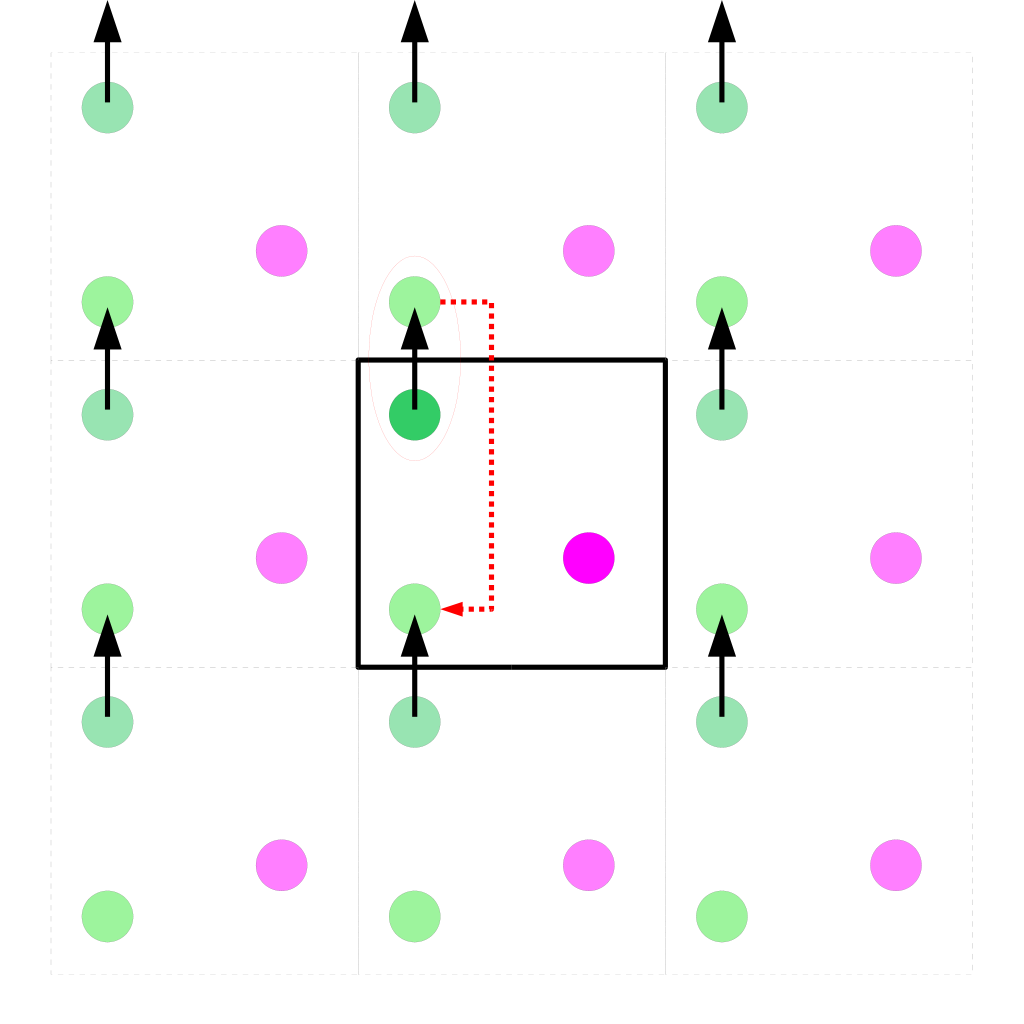
\includegraphics[width=0.7\textwidth, trim=0cm 0cm 0cm 0cm]{DSMC/figures/periodic_boundary_conditions.png}
\end{center}
\caption{Periodic boundary conditions allows particlez ta fly outta a system by re-enterin it up in tha opposite side. This reduces tha amount of finite size system effects, n' you can put dat on yo' toast. Image from \url{http://en.wikipedia.org/wiki/File:Limiteperiodicite.svg}, accessed 16 March, 2014.}
\label{fig:dsmc_periodic_boundary_conditions}
\end{figure}
Da state of a DSMC simulation is straight-up busted lyrics bout by tha $6M$ phase variables, three velocitizzles n' three positions per simulated particle.

Since our phat asses aint gots detailed shiznit bout tha positionz of all tha real atoms, we cannot calculate tha forces between tha particles. Instead, we assume dat tha gas particlez only undergo binary collisions (we neglect collisions between three or mo' particles), just like our phat asses did while derivin tha Boltzmann equation up in section \ref{sec:boltzmann_equation}. Particlez is sorted tha fuck into collision cells before tha collisions is performed up in a stochastic manner, where tha rate of collisions n' post-collision velocitizzles is determined from kinetic theory. We can be thinkin dat tha collision step up in tha model be a operator, a stochastic function $\mathcal{C}(\vec r, \vec v, \mathcal{G})$, where $\vec r$ n' $\vec v$ form tha phase space point n' $\mathcal G$ gotz nuff all shiznit bout tha system geometry. Do not worry, dis is ghon be clear up in a minute.\\
Da equationz of motion is integrated by applyin tha standard Eula method on tha positions so dat $\vec r_i(t+\Delta t) = \vec r_i(t) + \vec v_i(t)\Delta t$ fo' particle $i$. Da timestep is chosen lil' small-ass enough so dat we can split it tha fuck into two parts; movin n' colliding. This be a reasonable assumption as long as tha timestep $\Delta t$ is smalla than tha mean collision time $\tau_\text{coll}$ (equation \eqref{eq:kinetic_theory_mean_collision_time})
\begin{align}
	\Delta t \leq \tau_\text{coll} = \frac{1}{\sqrt 2 \pi d^2 \rho_n \langle v \rangle},
\end{align}
since tha velocitizzle then do not chizzle durin tha timestep. If a particle interacts wit a funky-ass boundary durin tha timestep, some sort of surface interaction rule be applied before tha timestep is continued (we allow a particle ta collide wit tha surface nuff muthafuckin times durin a single timestep).

Da movin step can also be peeped as a stochastic operator, $\mathcal{M}(\vec r, \vec v, \mathcal{G})$ since tha surface interaction often be a stochastic process. Different surface interaction models is discussed up in section \ref{sec:surface_interactions} wit a thugged-out detailed description of tha implementation up in section \ref{sec:dsmc_complex_geometries}. Right back up in yo muthafuckin ass. Statistical propertizzles is sampled all up in tha end of each timestep where tha physical quantitizzles is sampled as time averages fo' realz. A flow chart illustratin tha stepz of a typical DSMC algorithm is presented up in figure \ref{fig:dsmc_flowchart}.
\begin{figure}[ht]
\begin{center}
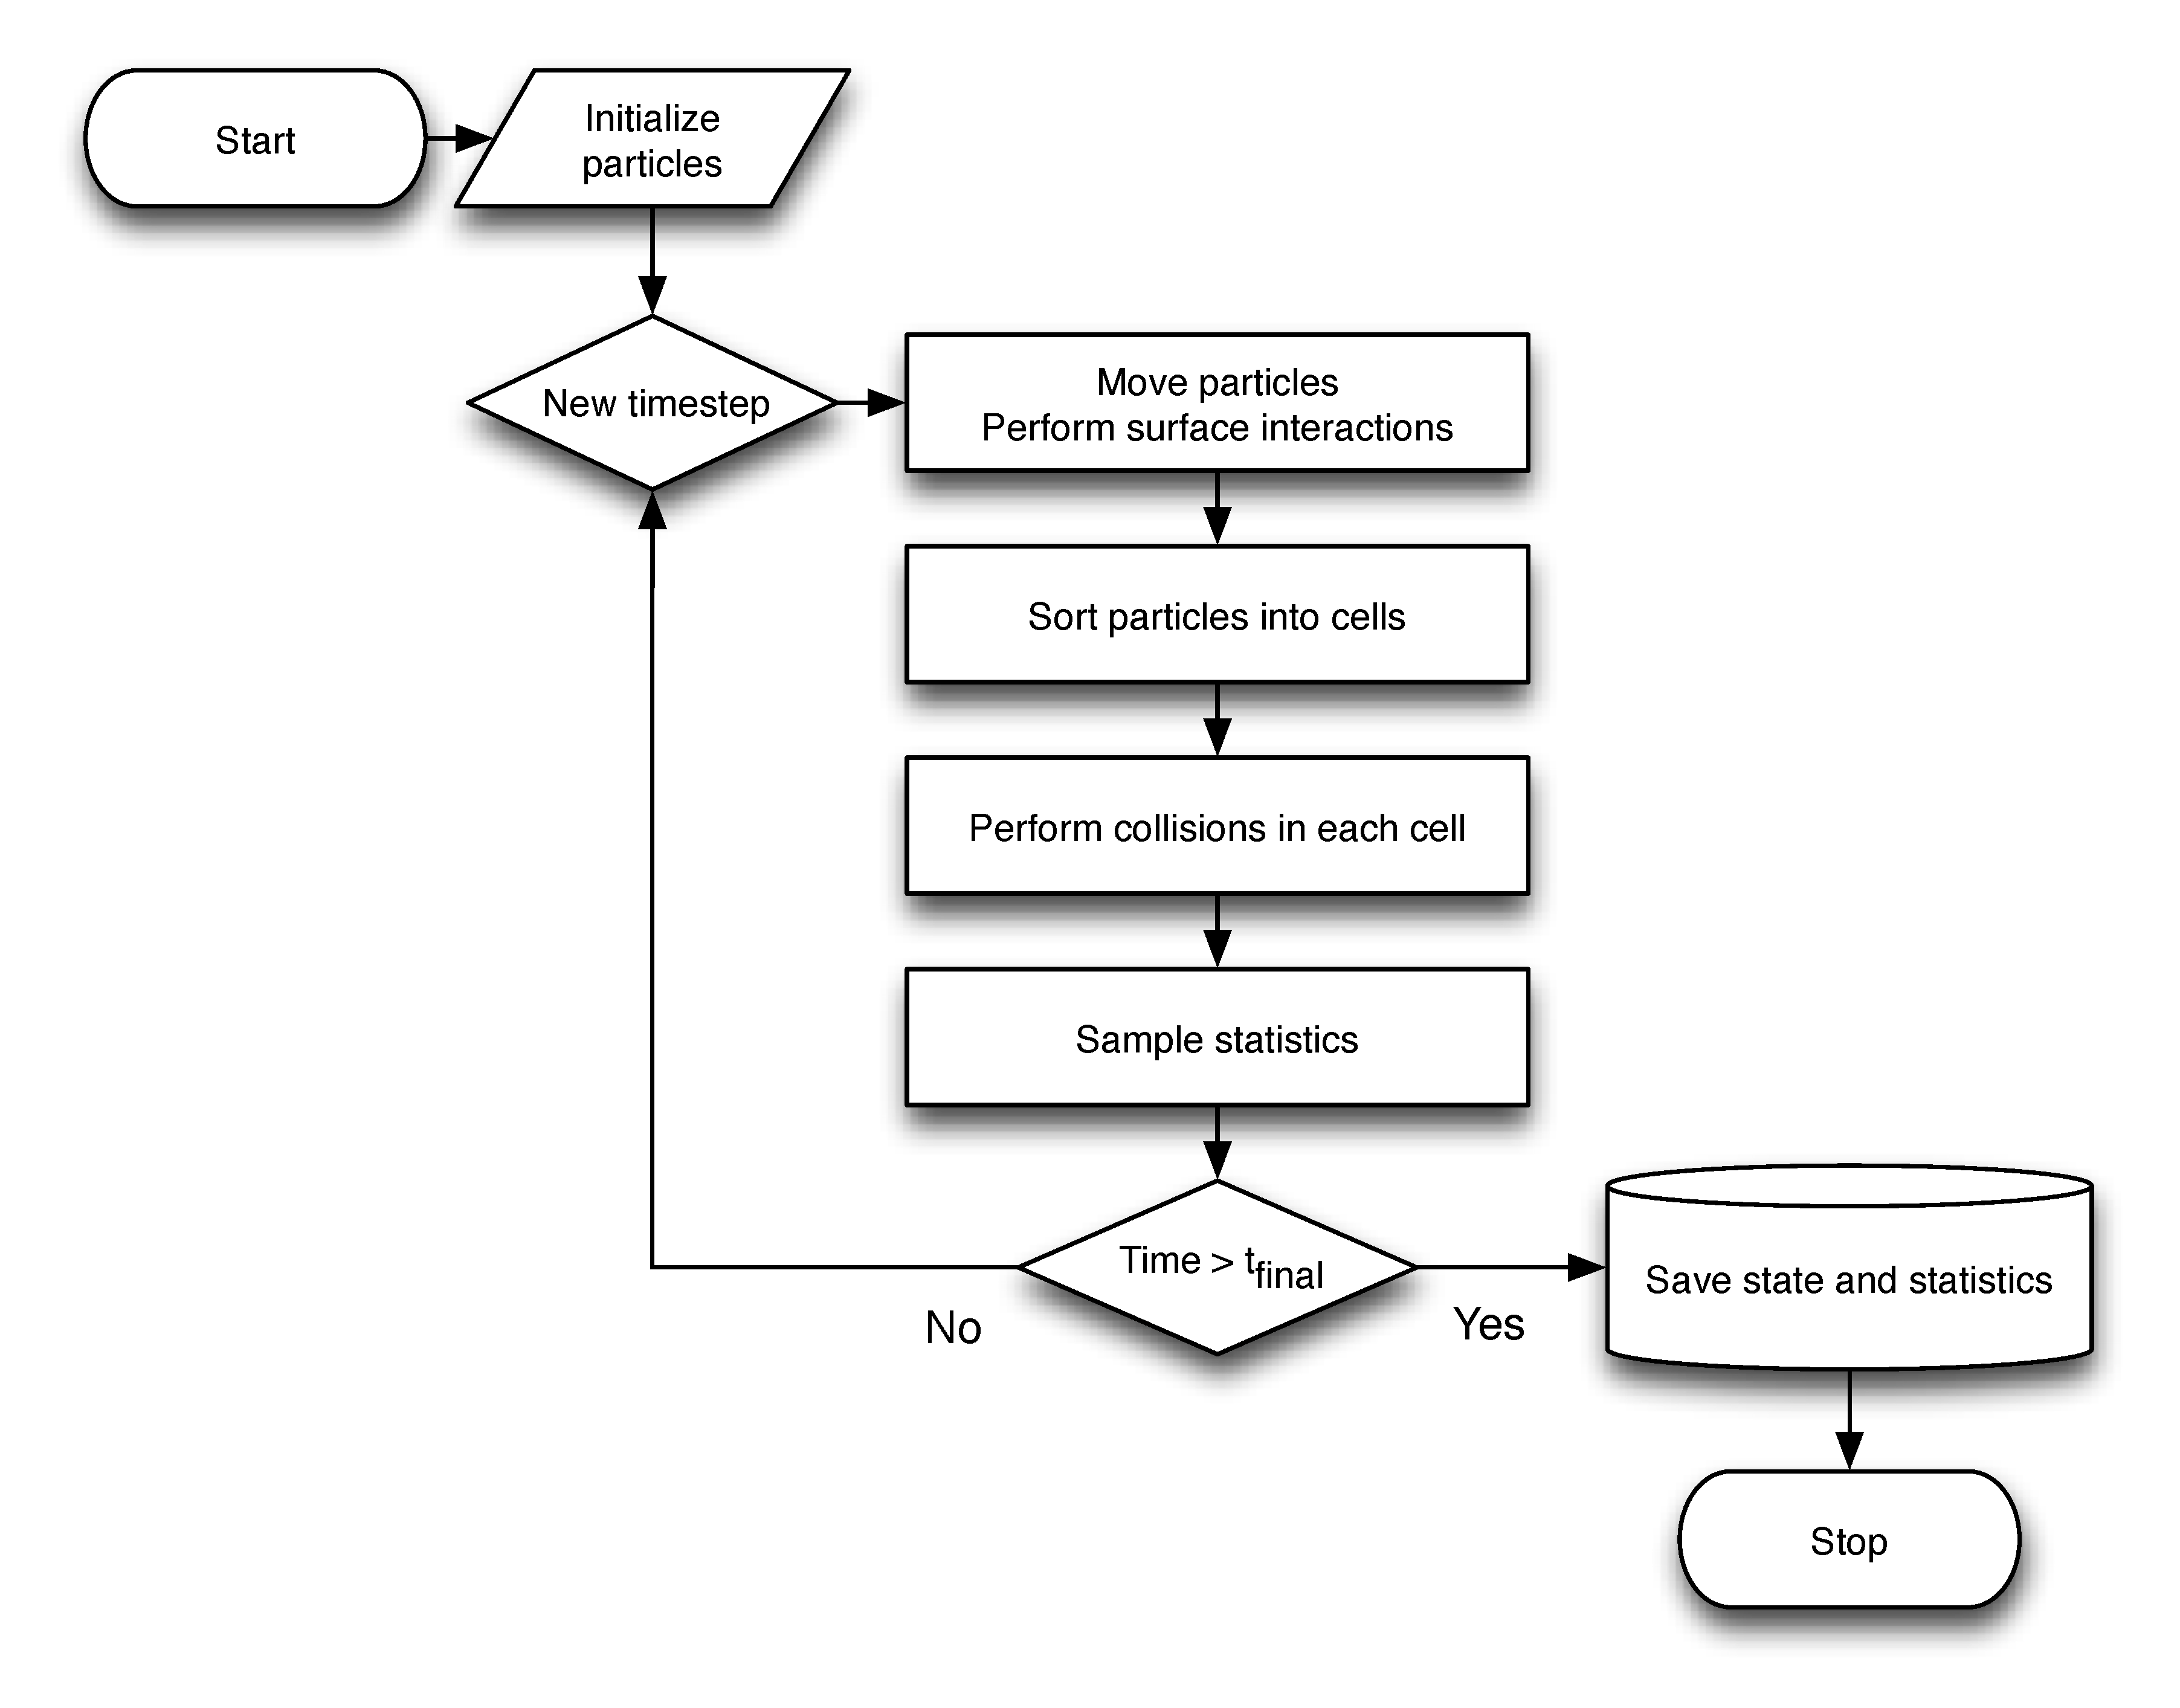
\includegraphics[width=\textwidth, trim=0cm 0cm 0cm 0cm, clip]{DSMC/figures/dsmc_flowchart.eps}
\end{center}
\caption{Typical steps fo' a DSMC algorithm.}
\label{fig:dsmc_flowchart}
\end{figure}

